\section{Lezione 13 - Support Vector Machine}\label{lezione-13---support-vector-machine}

Nelle precedenti puntate:

\begin{itemize}
\item
  Sappiamo che un iperpiano in uno spazio di dimensione \textit{m} ha VC
  dimension \textit{m+1}.
\item
  Si può aggiungere un vincolo di classificazione relativo al margine.
\item
  Per ottenere l'iperpiano con margine ottimo è necessario considerare
  l'ipotesi che minimizza la norma di \emph{w}.
\item
  Il tutto si fa prima con un polinomio di Lagrange e il suo duale.
\end{itemize}

\subsection{Dati non separabili linearmente}\label{dati-non-separabili-linearmente}

Tutto quello visto finora funziona se i dati sono linearmente
separabili.

Nel caso questi non lo siano è necessario aggiungere permettere che alcuni vincoli possano essere violati e per fare ciò vengono introdotte delle nuove variabili $\xi_i \geq 0$, una per ogni vincolo (ovvero per ogni esempio del training set), tale che:

$$ y_i (\vec{w} \cdot \vec{x}_i + b) \geq 1 - \xi_i $$

Queste nuove variabili rappresentano la distanza dell'esempio \textit{i}-esimo dal margine.

\begin{figure}[htbp]
\centering
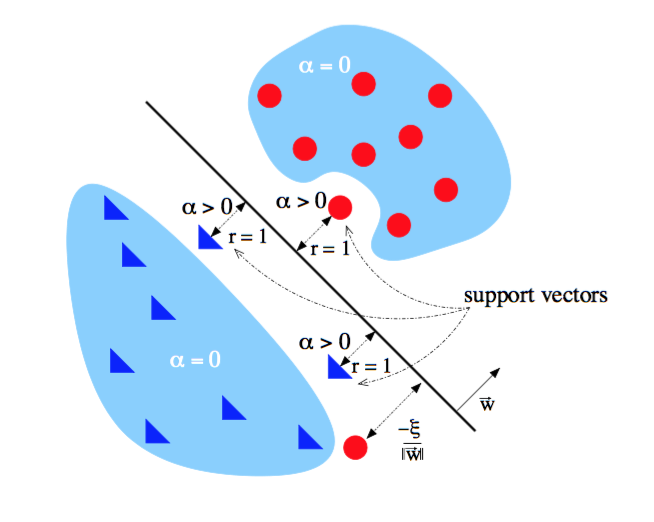
\includegraphics[width = 0.6\textwidth]{./notes/immagini/l13-non-linear.png}
\caption{SVM con dati non linearmente separabili.}
\end{figure}

L'idea è quindi quella di andare a sommare alla funzione costo la sommatoria di tutti i $\xi_i$ dei vari esempi presenti nel training set, moltiplicata per un coefficiente di penalizzazione \textit{C} che rappresenta un iper-parametro dell'algoritmo di apprendimento, da ottimizzare con le tecniche di model selection.

La nuova formula da minimizzare diventa:

$$ \frac{1}{2}||\vec{w}||^2 + C \sum\limits_{i=1}^n \xi_i $$

In pratica vengono penalizzati (aumentato il costo) gli esempi che non rispettano il margine.

La minimizzazione avviene considerano il problema duale, che risulta essere definito come:

$$max_\alpha \sum\limits_{i=1}^n \alpha_i - \frac{1}{2}\sum\limits_{i,j = 1}^n y_i y_j \alpha_i \alpha_j (\vec{x}_i \cdot \vec{x}_j)$$

$$ \text{s.t.: } \forall i \in \{1, \ldots, n\} : 0 \leq \alpha_i \leq C \text{ e } \sum\limits_{i=1}^n y_i \alpha_i = 0$$

Da notare che le $\xi_i$ sono variabili del problema primale e che quindi non compaiono nel problema duale.

Questa strategia per esempi non linearmente separabili non sempre
garantisce buone prestazioni perché un iper-piano può solo rappresentare
dicotomie dello spazio delle istanze.

Per questo motivo, quando gli esempi non sono linearmente separabili su
usa una strategia divisa in due passi:

\begin{enumerate}
\item
  Si mappano i dati di ingresso (input space) in uno spazio a dimensione
  molto superiore (feature space). Quindi a partire dalle feature degli
  elementi dell'input space vengono creati nuovi esempi nel feature
  space che utilizza combinazioni non lineari delle feature del primo
  spazio.
\item
  Si calcola poi l'iper-piano ottimo per il nuovo spazio usando la
  formulazione precedente (che prende il nome di variabili slack).
\end{enumerate}

Perché dovrei farlo?

\begin{enumerate}
\item
  Perché il \textbf{teorema sulla separabilità di Cover} afferma che un problema di classificazione complesso, formulato
  attraverso una trasformazione non lineare dei dati in uno spazio ad
  alta dimensionalità, ha maggiore probabilità di essere linearmente
  separabile che in uno spazio a bassa dimensionalità).
\item
  Perché l'iper-piano ottimo minimizza la VC-Dimension e quindi la
  capacità di generalizzazione migliora.
\end{enumerate}

Viene quindi utilizzata una trasformazione $\varphi(\cdot)$ non lineare, da applicare ai dati originari del problema $\{(\vec{x}_i, y_i)\}_1^n$ tale che:

$$ \forall i \: \vec{x}_i \in R^m, \varphi(\vec{x}_i) = \vec{Z}, \vec{Z} \in R^M, M \gg m $$

Il vettore ottenuto può essere rappresentato come $\vec{\varphi}(\vec{x}) = [ \varphi_1(\vec{x}), \ldots , \varphi_M(\vec{x}) ] $.

Con questa notazione è possibile andare a definire l'iper-piano nel nuovo spazio con:

$$ \sum\limits_{j=1}^M w_j \varphi_j(\vec{x}) + b = 0$$

che se si considera il termine noto $b = w_0$ e si aggiunge $\varphi_0(\vec{x}) = 1$, risulta essere

$$ \sum\limits_{j=0}^M w_j \varphi_j(\vec{x}) = \vec{w} \cdot \vec{\varphi}(\vec{x}) = 0$$

Andando a sostituire il $\vec{w}$ dell'equazione precedente con $ \vec{w} = \sum\limits_{k=1}^n j_k \alpha_k \vec{\varphi}(\vec{x})$ si ottiene:

$$ \sum\limits_{j=1}^M w_j \varphi(\vec{x_k}) \cdot \varphi(\vec{x}) = 0 $$

Con il termine $\varphi(\vec{x}) \cdot \varphi(\vec{x})$ rappresenta il prodotto scalare tra un vettore del training set $\vec{x}_k$ e il vettore in input $\vec{x}$ calcolato nello spazio $R^M$.

\subsection{Funzioni Kernel}\label{funzioni-kernel}

Lo spazio di dimensione superiore serve solo per calcolare il prodotto scalare tra i due vettori, si può quindi definire una funzione $K(\cdot, \cdot)$ che prende il nome di kernel e che calcola il prodotto scalare dei due vettori senza passare esplicitamente nello spazio di dimensione superiore.

$$ K(\vec{x}_k, \vec{x}) = \varphi(\vec{x}) \cdot \varphi(\vec{x})$$

Assumendo di avere una di queste funzioni, il calcolo del vettore $\vec{w}$ diventa:

$$ \vec{w} = \sum\limits_{k=1}^n j_k y_k \alpha_k K(\vec{x}_k, \vec{x}) $$

Per il teorema di Mercer esistono delle funzioni di questo tipo, ma è necessario che soddisfino determinate condizioni.

Alcune di queste sono:

\begin{itemize}
\item \textbf{Polinomiale di grado \textit{p}}: $K(\vec{x},\vec{y}) = (\vec{x} \cdot \vec{y} +1) ^p$
\item \textbf{RBF}: $ K(\vec{x},\vec{y}) = exp(-\frac{1}{2\sigma^2}||\vec{x}-\vec{y}||^2)$
\end{itemize}

La formulazione duale del problema risulta quindi essere:

$$max_\alpha \sum\limits_{i=1}^n \alpha_i - \frac{1}{2}\sum\limits_{i,j = 1}^n y_i y_j \alpha_i \alpha_j K(\vec{x}_i ,\vec{x}_j)$$

$$ \text{s.t.: } \forall i \in \{1, \ldots, n\} : 0 \leq \alpha_i \leq C \text{ e } \sum\limits_{i=1}^n y_i \alpha_i = 0$$

Per fare la classificazione viene utilizzato il \textbf{segno} della funzione:

\begin{align*}
f(\vec{u})  &= \sum\limits_{i = 1}^n y_i  \alpha_i  K(\vec{x}_i,  \vec{u}) + b
\end{align*}

\subsection{Regressione}\label{regressione}

Quando si considera il problema di approssimazione di funzioni a valori
reali (regressione) si utilizza l'$\epsilon$-tubo: output che differiscono dai
valori di target per più di $\epsilon$ in valore assoluto vengono penalizzati
linearmente, altrimenti non vengono considerati errori. In pratica
aggiungo un intervallo di tolleranza al iper-piano che partiziona lo
spazio.

\begin{figure}[htbp]
\centering
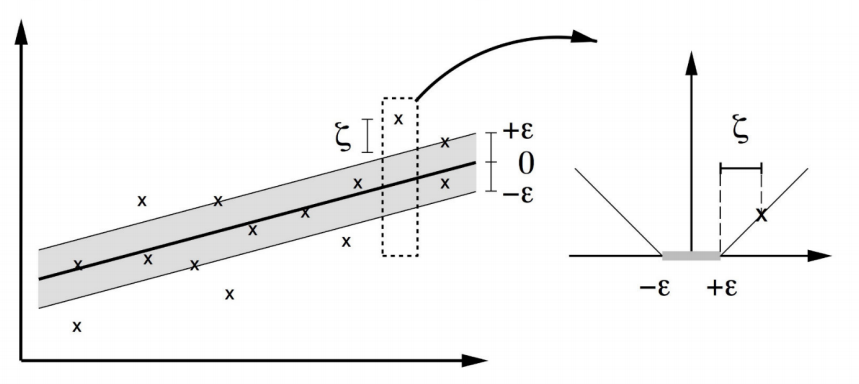
\includegraphics[width = 0.8\textwidth]{./notes/immagini/l13-primale-duale.png}
\caption{Regressione in forma primale (a sinistra) e duale (a destra)}
\end{figure}

\todo[inline]{Mancano formule (ultime due slide) http://www.math.unipd.it/\~{}aiolli/corsi/1516/aa/SVM.pdf}